\documentclass[12pt]{article}
\usepackage[T1, T2A]{fontenc}
\usepackage[utf8]{inputenc}
\usepackage[russian]{babel}
\usepackage{hyperref}
\usepackage{graphicx}
\graphicspath{ {../Images/} }

\author{Григорий Матюхин}
\date{\today}
\title{Лабораторная работа \textnumero9.\\Управление \texttt{SELinux}}

\begin{document}
\maketitle
\newpage
\tableofcontents
\newpage
\section{Цель работы}
Получить навыки работы с контекстом безопасности и политиками \texttt{SELinux}.

\section{Последовательность выполнения работы}
\subsection{Управление режимами SELinux}
\begin{enumerate}
	\item Запустите терминал и получите полномочия администратора:
	\item Просмотрите текущую информацию о состоянии \texttt{SELinux}:
	      \\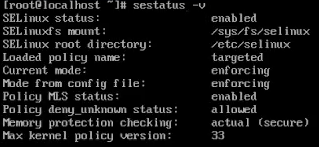
\includegraphics{1.png}
	\item Посмотрите, в каком режиме работает \texttt{SELinux}:
	      \\
\includegraphics{2.png}
	\item Измените режим работы \texttt{SELinux} на разрешающий (\texttt{Permissive}):
	      \\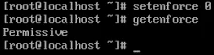
\includegraphics{3.png}
	\item В файле \texttt{/etc/sysconfig/selinux} с помощью редактора установите \texttt{SELINUX=disabled}. Перезагрузите систему.
	      \\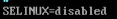
\includegraphics{4.png}
	\item После перезагрузки запустите терминал и получите полномочия администратора.
	\item Посмотрите статус \texttt{SELinux}:
	      \\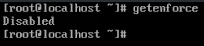
\includegraphics{5.png}
	\item Попробуйте переключить режим работы \texttt{SELinux}:
	      \\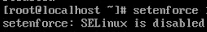
\includegraphics{6.png}
	\item Откройте файл \texttt{/etc/sysconfig/selinux} с помощью редактора и установите \texttt{SELINUX=enforcing}. Перезагрузите систему.
	      \\
\includegraphics{7.png}
	\item Во время загрузки системы вы, скорее, всего получите предупреждающее сообщение о необходимости восстановления меток \texttt{SELinux}, что может занять некоторое время, а также потребует дополнительной перезагрузки системы.
	\item После перезагрузки в терминале с полномочиями администратора просмотрите текущую информацию о состоянии \texttt{SELinux}. Убедитесь, что система работает в принудительном режиме (\texttt{enforcing}) использования \texttt{SELinux}.
	      \\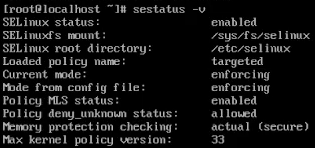
\includegraphics{8.png}
\end{enumerate}

\subsection{Использование restorecon для восстановления контекста безопасности}
\begin{enumerate}
	\item Запустите терминал и получите полномочия администратора.
	\item Посмотрите контекст безопасности файла \texttt{/etc/hosts}:
	      \\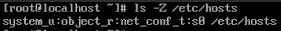
\includegraphics{9.png}
	\item Скопируйте файл \texttt{/etc/hosts} в домашний каталог. Проверьте контекст файла \texttt{~/hosts}:
	      \\
\includegraphics{10.png}
	\item Попытайтесь перезаписать существующий файл \texttt{hosts} из домашнего каталога в каталог \texttt{/etc}:
	\item Убедитесь, что тип контекста по-прежнему установлен на \texttt{admin\_home\_t}:
	      \\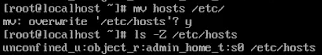
\includegraphics{11.png}
	\item Исправьте контекст безопасности:
	\item Убедитесь, что тип контекста изменился:
	      \\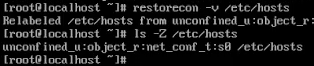
\includegraphics{12.png}
	\item Для массового исправления контекста безопасности на файловой системе введите \texttt{touch /.autorelabel} и перезагрузите систему. Во время перезапуска не забудьте нажать клавишу \texttt{Esc} на клавиатуре, чтобы вы видели загрузочные сообщения. Вы увидите, что файловая система автоматически перемаркирована.
	      \\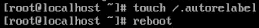
\includegraphics{13.png}
	      \\
\includegraphics{14.png}
\end{enumerate}

\subsection{Настройка контекста безопасности для нестандартного расположения файлов веб-сервера}
\begin{enumerate}
	\item Запустите терминал и получите полномочия администратора.
	\item Установите необходимое программное обеспечение:
	      \\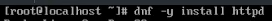
\includegraphics{15.png}
	      \\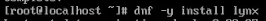
\includegraphics{15_1.png}
	\item Создайте новое хранилище для файлов web-сервера:
	      \\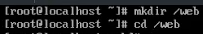
\includegraphics{16.png}
	\item Создайте файл \texttt{index.html} в каталоге с контентом веб-сервера \texttt{Welcome to my web-server}
	\item В файле \texttt{/etc/httpd/conf/httpd.conf} закомментируйте строку \texttt{DocumentRoot "/var/www/html"} и ниже добавьте строку \texttt{DocumentRoot "/web"} Затем в этом же файле ниже закомментируйте раздел \\
	      \begin{verbatim}
          <Directory "/var/www">
            AllowOverride None
            Require all granted
          </Directory>
        \end{verbatim}
	      и добавьте следующий раздел, определяющий правила доступа \\
	      \begin{verbatim}
          <Directory "/web">
            AllowOverride None
            Require all granted
          </Directory>
        \end{verbatim}
	      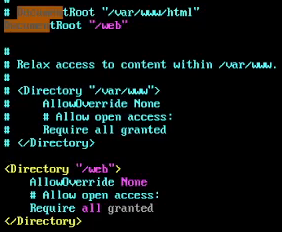
\includegraphics{17.png}
	\item Запустите веб-сервер и службу \texttt{httpd}:
	      \\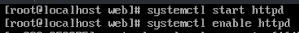
\includegraphics{18.png}
	\item В терминале под учётной записью своего пользователя обратитесь к веб-серверу в текстовом браузере \texttt{lynx}:
	      \\
\includegraphics{19.png}
	\item В терминале с полномочиями администратора переключите \texttt{SELinux} в разрешающий режим:
	      \\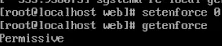
\includegraphics{20.png}
	\item В терминале под учётной записью своего пользователя снова обратитесь к веб-серверу:
	      \\
\includegraphics{21.png}
	\item В терминале с полномочиями администратора примените новую метку контекста к \texttt{/web}:
	      \\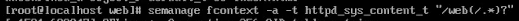
\includegraphics{22.png}
	\item Восстановите контекст безопасности:
	\item Установите \texttt{SELinux} в режим принудительного исполнения:
	      \\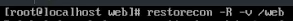
\includegraphics{23.png}
	\item В терминале под учётной записью своего пользователя снова обратитесь к веб-серверу. Теперь вы получите доступ к своей пользовательской веб-странице.
	      \\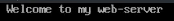
\includegraphics{24.png}
\end{enumerate}

\subsection{Работа с переключателями SELinux}
\begin{enumerate}
	\item Запустите терминал и получите полномочия администратора.
	\item Посмотрите список переключателей \texttt{SELinux} для службы \texttt{ftp}:
	      \\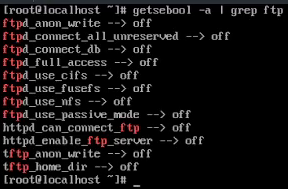
\includegraphics{25.png}
	\item Для службы \texttt{ftpd\_anon} посмотрите список переключателей с пояснением, за что отвечает каждый переключатель, включён он или выключен:
	\item Измените текущее значение переключателя для службы \texttt{ftpd\_anon\_write} с \texttt{off} на \texttt{on}:
	\item Повторно посмотрите список переключателей \texttt{SELinux} для службы \texttt{ftpd\_anon\_write}:
	\item Посмотрите список переключателей с пояснением:
	\item Измените постоянное значение переключателя для службы \texttt{ftpd\_anon\_write} с \texttt{off} на \texttt{on}:
	\item Посмотрите список переключателей:
	      \\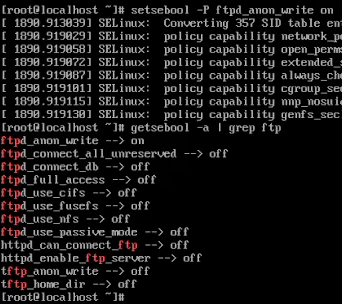
\includegraphics{26.png}
\end{enumerate}

\section{Контрольные вопросы}
\begin{enumerate}
	\item Вы хотите временно поставить \texttt{SELinux} в разрешающем режиме. Какую команду вы используете? \\
	      \texttt{setenforce 0}
	\item Вам нужен список всех доступных переключателей \texttt{SELinux}. Какую команду вы используете? \\
	      \texttt{getsebool -a}
	\item Каково имя пакета, который требуется установить для получения легко читаемых сообщений журнала \texttt{SELinux} в журнале аудита? \\
	      \texttt{setroubleshoot-server}
	\item Какие команды вам нужно выполнить, чтобы применить тип контекста \texttt{httpd\_sys\_content\_t} к каталогу \texttt{/web}? \\
	      \begin{enumerate}
		      \item Применить новую метку контекст к \texttt{/web}: \\
		            \texttt{semanage fcontext -a -t httpd\_sys\_content\_t "/web(/.*)?"}
		      \item Восстановить контекст безопасности: \\
		            \texttt{restorecon -R -v /web}
	      \end{enumerate}
	\item Какой файл вам нужно изменить, если вы хотите полностью отключить \texttt{SELinux}? \\
	      \texttt{/etc/sysconfig/selinux}
	\item Где \texttt{SELinux} регистрирует все свои сообщения? \\
	      \texttt{/var/log/audit/audit}
	\item Вы не знаете, какие типы контекстов доступны для службы \texttt{ftp}. Какая команда позволяет получить более конкретную информацию? \\
	      \texttt{man file\_contexts} \\
	      \texttt{man default\_contexts}
	\item Ваш сервис работает не так, как ожидалось, и вы хотите узнать, связано ли это с \texttt{SELinux} или чем-то ещё. Какой самый простой способ узнать? \\
	      Отключить \texttt{SELinux} и проверить работы сервиса еще раз.
\end{enumerate}

\section{Вывод}
В ходе выполнения данной работы я получил навыки работы с контекстом безопасности и политиками \texttt{SELinux}.

\end{document}
